\documentclass{article}
\usepackage{graphicx}
\usepackage{xcolor}
\usepackage{amsmath}
\usepackage{amssymb}
\usepackage{authblk}
\usepackage{subcaption}
\usepackage{float}
\usepackage{placeins}
\usepackage{booktabs}
\usepackage{pdflscape}
\usepackage[numbers]{natbib}
\usepackage{setspace}
\usepackage{parskip}
\usepackage{microtype}
\usepackage[margin=2.5cm]{geometry}

\setlength{\parindent}{0pt}
\setlength{\parskip}{7pt}
\linespread{1.15}

% PCA variance -- taken directly from Figure 4
\newcommand{\PCAVarI}{46.8\%}
\newcommand{\PCAVarII}{28.0\%}
\newcommand{\PCAVarTotal}{74.8\%}

\title{\textbf{Neural Population Dynamics Reveal Internal Representations
Underlying Adaptive Obstacle Avoidance in Reinforcement Learning}}

\author[1]{Peter Ohue}
\author[1]{Emily Oby}
\author[1,2]{Gunnar Blohm}

\affil[1]{Centre for Neuroscience Studies, Queen's University, ON, Canada}
\affil[2]{Department of Biomedical and Molecular Sciences,
          Queen's University, ON, Canada}

\date{}

\begin{document}

\maketitle

%--------------------------------------------------------------
\begin{abstract}
%--------------------------------------------------------------

When a controller must steer toward a goal while unexpected forces deflect
its path, what determines whether it recovers or fails?
This question sits at the intersection of motor neuroscience and autonomous
control, and it remains difficult to answer from behavioural data alone
because the internal signals that drive moment-to-moment corrections are
not directly observable.
We developed a computational framework that places a reinforcement learning
controller -- trained through the same kind of trial-and-error refinement
that shapes biological motor learning -- in a reaching-inspired
obstacle-avoidance task and perturbs it with graded lateral force impulses,
mirroring protocols used to study feedback control in human arm movements.
Rather than reporting only task success, we treat the controller's
hidden-layer activity as a neural population recording and apply
dimensionality reduction, state-space trajectory analysis, and linear
decoding to ask what internal representations track behaviour and
distinguish recovery from failure.

We find that the controller adapts successfully to moderate perturbations
across all directions but fails progressively under strong rightward
disturbances, revealing a direction-dependent asymmetry in robustness.
The hidden-layer activity organises into a compact low-dimensional manifold
-- accounting for the majority of population variance in just two
dimensions -- and subdivides into discrete clusters that align with phases
of the movement rather than with specific perturbation conditions.
Lateral velocity is clearly encoded across the population, and the most
extreme perturbation conditions produce latent states that a simple linear
classifier can separate from one another, whereas mild conditions remain
geometrically indistinct.
These properties closely mirror those documented in motor cortex during
biological reaching: compact manifold geometry, phase-structured clustering,
and distributed encoding of kinematic variables.
Our results suggest that reward-driven optimisation spontaneously generates
representational organisation similar to biological motor populations, and
that population-style analyses of artificial controllers can reveal not just
whether adaptive behaviour succeeds but why it sometimes does not.

\end{abstract}

%==============================================================
\section{Introduction}
%==============================================================

The ability to reach toward a target while correcting for unexpected
disturbances is a hallmark of biological motor control
\citep{Pruszynski2012,Nashed2014,Dimitriou2013,Scott2004}.
When the arm is pushed mid-flight, the nervous system does not wait for a
deliberate decision; corrections emerge within tens of milliseconds,
shaped by the continuous interplay between sensory feedback and internal
predictions \citep{Todorov2002,Todorov2009,Codol2023}.
These fast, flexible responses arise from coordinated activity across
distributed neural populations in motor cortex and cerebellum rather than
from single-neuron specialisation
\citep{Churchland2012,Shenoy2013,Gallego2017,Crevecoeur2019}.
Understanding how population-level organisation gives rise to robust
adaptive behaviour is a central goal of systems motor neuroscience.

Reinforcement learning (RL) offers a complementary perspective.
In RL, a controller is not designed with explicit rules; instead, it
discovers its own movement strategy through repeated interaction with the
environment, receiving a reward signal whenever it performs well and
adjusting accordingly \citep{Kaelbling1996RLSurvey,SuttonBarto2018}.
This is, in spirit, how biological motor skill is acquired: practice
generates outcome feedback, and the nervous system gradually updates its
internal policy to maximise success \citep{Oby2019,Mathis2024}.

\paragraph{What is PPO, and why does it matter here?}

The specific algorithm we use is Proximal Policy Optimization (PPO)
\citep{Schulman2017}.
For readers more at home in a neuroscience lab than a machine learning
classroom, the clearest analogy is incremental motor learning.
Imagine a participant practising a novel reaching task: each trial, the
motor system asks whether the movement was better or worse than usual, and
nudges the control policy slightly toward strategies that worked.
Experienced clinicians and motor learning researchers know that
overcorrecting after a single poor trial is counterproductive -- it
destabilises what already works.
PPO builds this conservatism into its update rule.
After each batch of training trials, it computes how much better or worse
the new strategy would have performed relative to the old one, then
limits the size of the update so the policy never changes too drastically
in a single step.
This is the meaning of ``proximal'': the new policy stays close to the
current one, much as incremental motor learning keeps refined movements
anchored to the existing motor programme.
The result is a learner that improves steadily without the wild swings
in performance that unconstrained gradient updates can produce.

Most RL studies evaluate controllers solely on task outcomes -- goal
success rate, cumulative reward -- while treating the network as a black
box \citep{Rudin2019,Molnar2022}.
This is informative but incomplete: knowing that a controller succeeds
nine times out of ten tells you nothing about what it does differently
on the tenth, or which internal signals predict whether a given
perturbation will be absorbed or cause failure.
The same interpretability problem motivates population analyses in
biological motor neuroscience: task performance measures confirm that a
subject compensates successfully, but the population dynamics reveal
\emph{how} and \emph{why} \citep{Churchland2012,Cunningham2014,Gallego2017}.

Recent work has shown that motor cortex activity during reaching unfolds
on low-dimensional neural manifolds -- smooth subspaces within the
high-dimensional activity space that capture the essential dynamics of
movement generation
\citep{Churchland2012,Shenoy2013,Cunningham2014,Gallego2017}.
These manifolds can be identified by principal component analysis (PCA),
their structure interrogated with trajectory analyses, and behaviourally
relevant variables decoded from them with linear classifiers
\citep{Cunningham2014,Oby2019,Blohm2009,Blohm2012}.
Whether an artificially trained controller develops similar organisation
is an open question with practical implications for interpretability
\citep{Bekkemoen2024XRL,TrimGrayston2024MechInterpRL}.

Here, we train a PPO controller on an obstacle-avoidance reaching task
and probe it with the same graded perturbation protocol used in biological
reaching experiments.
We record hidden-layer activity during evaluation and analyse it using
dimensionality reduction, trajectory visualisation, and linear decoding.
Our goal is to identify which representational features emerge from
reward-driven training, whether they parallel those in motor cortex, and
which features distinguish successful recovery from failure.

Our contributions are:
(i)~a population-analysis workflow applied to a trained RL controller
enabling direct comparison with biological motor data;
(ii)~evidence of compact low-dimensional manifold structure consistent
with neural manifold dynamics in motor cortex;
(iii)~identification of a direction-dependent asymmetry in robustness
visible in both behaviour and latent geometry; and
(iv)~demonstration that extreme perturbation conditions produce linearly
separable latent representations while mild conditions do not,
mirroring difficulty-dependent separability in biological populations.

%==============================================================
\section{Methodology}
%==============================================================

\subsection{Task Environment and State Representation}

We implemented the task using the Gymnasium interface
\citep{Towers2024Gymnasium}.
The agent is a two-dimensional point mass controlled by continuous force
commands, evolving under Newtonian dynamics.
Dynamics were kept deliberately minimal so that any representational
structure found in the network reflects learning rather than physical
constraints.
Figure~\ref{fig:schematic} shows the task schematically; Panel~A uses
a planar arm analogy for biological grounding, and all experiments use
the point-mass agent in Panel~C.

\begin{figure}[t]
  \centering
  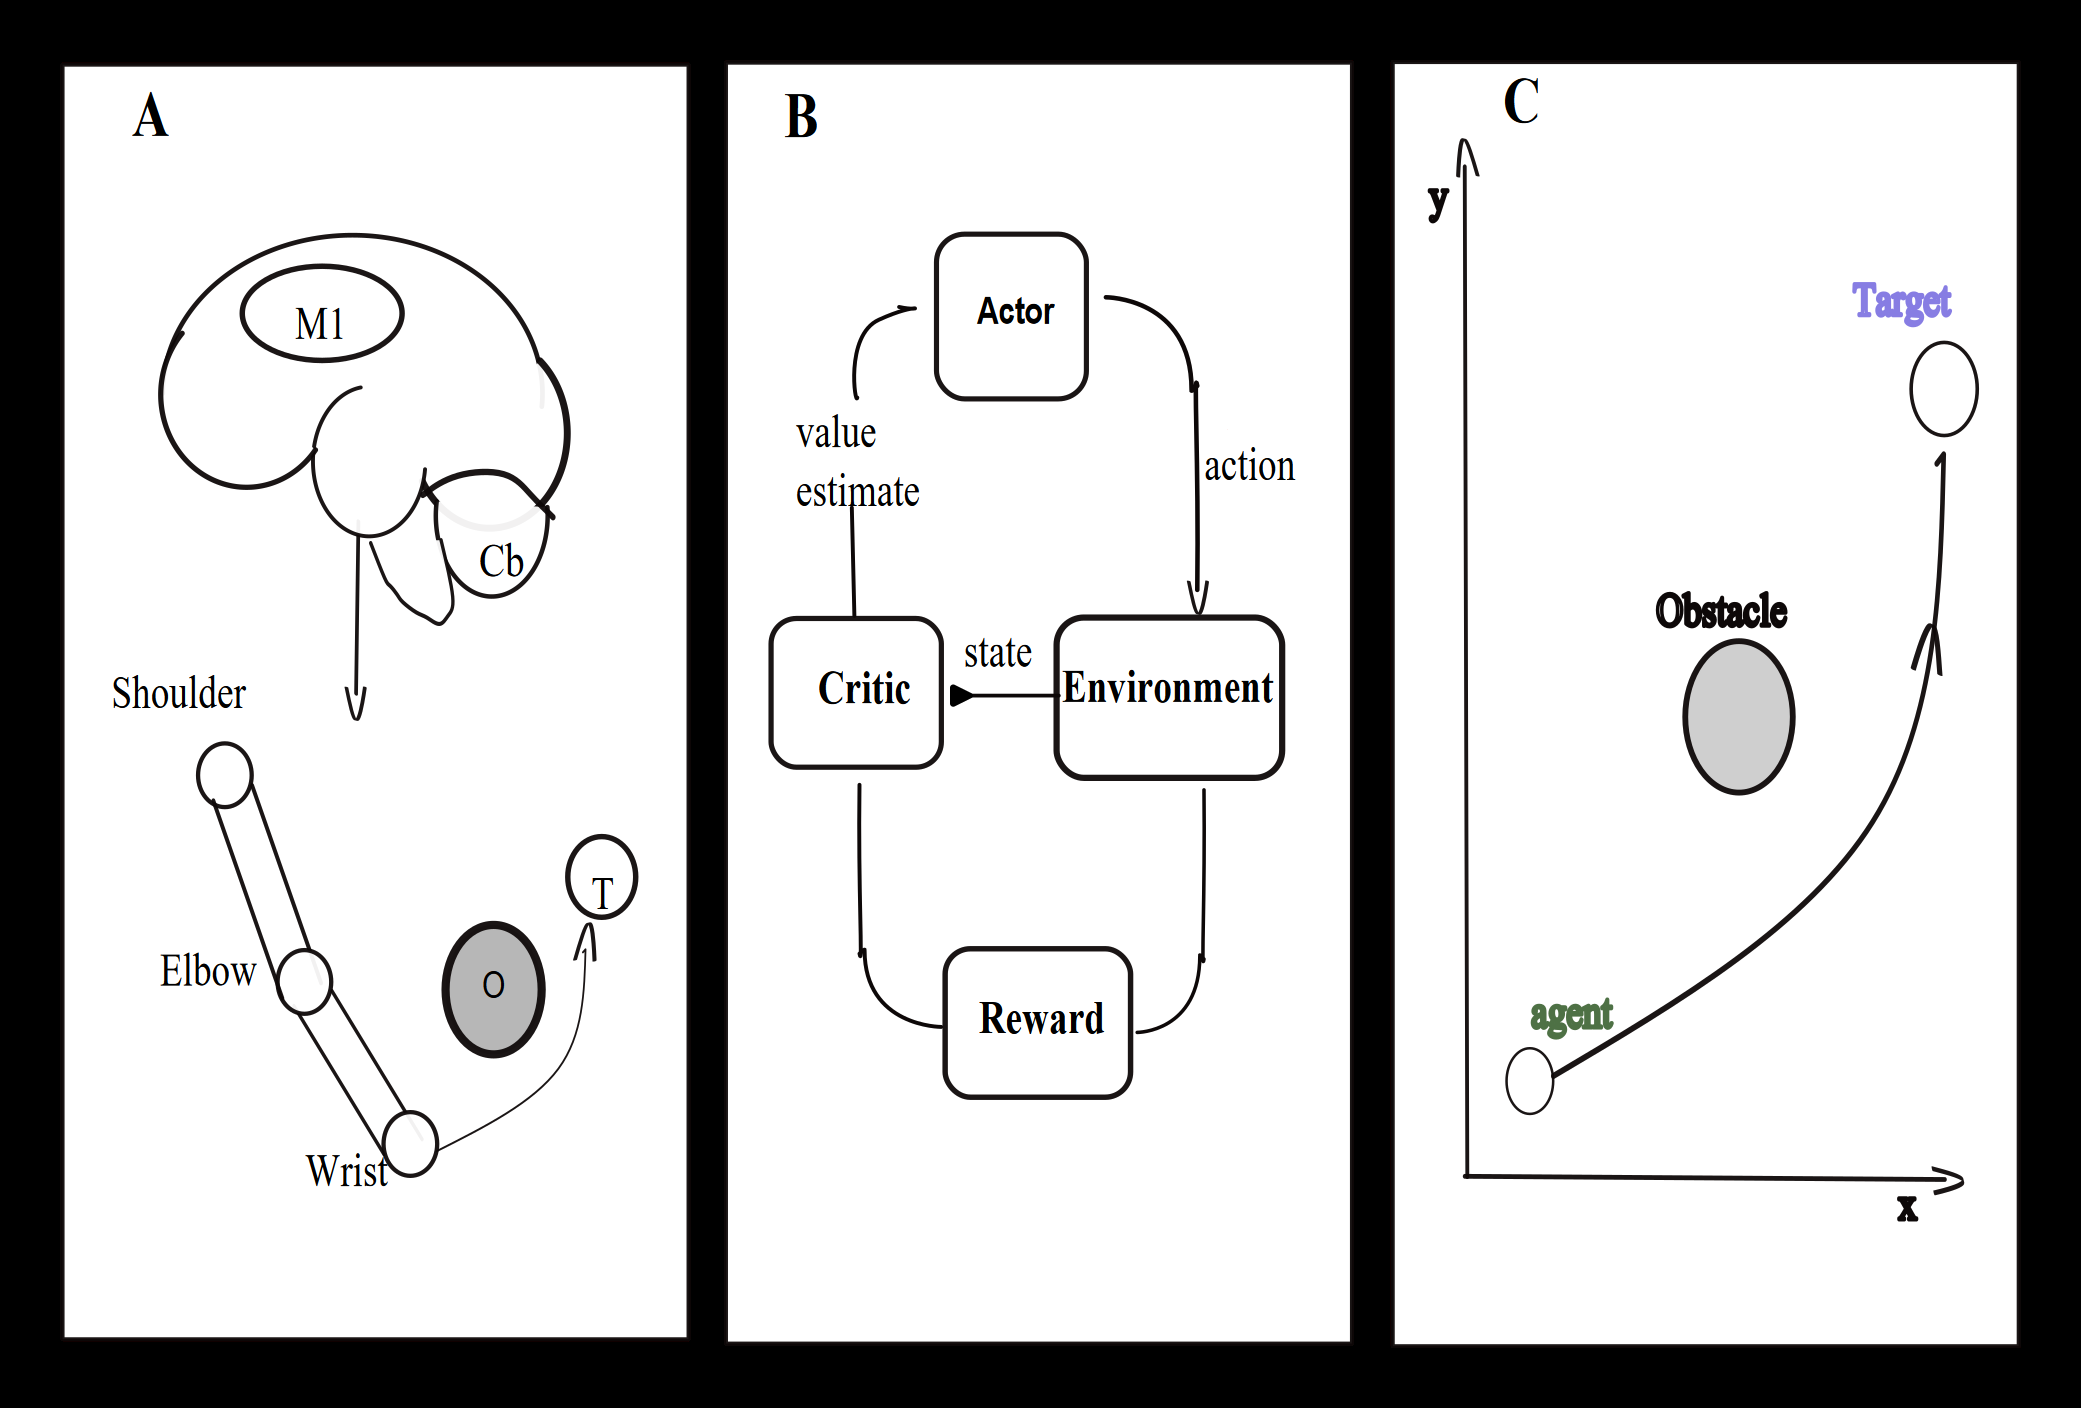
\includegraphics[width=0.88\linewidth]{fig1_schematic.png}
  \caption{\textbf{Task, control architecture, and analysis pipeline.}
    \textbf{(A)}~Biological analogy: motor cortex (M1) and cerebellum (Cb)
    drive a multi-joint arm toward a target (T) while avoiding an
    obstacle~(O). This panel is used for conceptual grounding; all
    experiments use a point-mass agent.
    \textbf{(B)}~The PPO actor--critic loop: the actor selects a
    continuous force command; the environment advances the agent and
    returns the next state; the critic estimates the long-term value of
    that state; a scalar reward drives both networks.
    \textbf{(C)}~Task geometry: the agent navigates from a fixed start
    through a two-obstacle corridor to a fixed goal on a 2-D plane.}
  \label{fig:schematic}
\end{figure}

The main experiment used a corridor formed by two static circular
obstacles.
A preliminary single-obstacle variant established the basic
obstacle-avoidance skill before the two-obstacle and perturbation
protocol were introduced.
The agent receives an agent-centred observation at each timestep:
\begin{equation}
  s_t = \bigl[
    g_x - x_t,\;g_y - y_t,\;
    o_{Lx} - x_t,\;o_{Ly} - y_t,\;
    o_{Rx} - x_t,\;o_{Ry} - y_t,\;
    v_{x,t},\;v_{y,t}
  \bigr]
  \label{eq:state}
\end{equation}
where $(x_t,y_t)$ is the agent's position, $(v_{x,t},v_{y,t})$ its
velocity, $(g_x,g_y)$ the goal, and $(o_L,o_R)$ the obstacle centres.

\subsection{Reward Structure and Perturbation Protocol}

The reward at each timestep balances four objectives:
\begin{equation}
  R_t = w_p\,\Delta d_{\mathrm{goal}}
        - w_v\,\|v_t\|
        - w_c\,C_t
        + w_s\,S_t
  \label{eq:reward}
\end{equation}
Progress toward the goal is rewarded; excessive speed penalised;
collision incurs a large negative penalty; reaching the goal earns a
terminal bonus.

Lateral force impulses were applied mid-movement for six timesteps:
\begin{equation}
  f_x(t) = p_i, \quad t \in [50,\,55], \quad
  p_i \in \{\pm0.15,\;\pm0.30,\;\pm0.45\}
  \label{eq:perturbation}
\end{equation}
defining seven conditions: control (P0) and three increasing leftward
(L1--L3) and three rightward (R1--R3) impulses.
The design mirrors perturbation protocols used in human reaching studies
to isolate online feedback correction
\citep{Pruszynski2012,Nashed2014,Dimitriou2013,Todorov2002}.

\subsection{Reinforcement Learning Controller}

All training used Stable-Baselines3 \citep{Raffin2021StableBaselines3}
with PPO \citep{Schulman2017}.
PPO maximises a clipped surrogate objective:
\begin{equation}
  L^{\mathrm{CLIP}}(\theta) = \mathbb{E}_t\!\Bigl[
    \min\!\bigl(r_t(\theta)\hat{A}_t,\;
    \mathrm{clip}(r_t(\theta),1-\epsilon,1+\epsilon)\hat{A}_t\bigr)
  \Bigr]
  \label{eq:ppo}
\end{equation}
where $r_t(\theta)$ is the probability ratio of updated to old policy,
$\hat{A}_t$ the estimated advantage, and $\epsilon=0.2$ the clipping
threshold.

The controller uses separate policy and value networks, each a feedforward
MLP with two hidden layers of 256 units.
Continuous actions are drawn from a diagonal Gaussian; observations were
normalised online (VecNormalize).
Training ran for $2\times10^6$ timesteps with learning rate $3\times10^{-4}$,
discount $\gamma=0.99$, entropy coefficient $0.005$, value-function
coefficient $0.5$, and gradient norm clipped at $0.5$.
All experiments used Stable-Baselines3 v2.8.0, Gymnasium, and PyTorch
on an Intel\textregistered\ Core\textsuperscript{TM} Ultra~7~255H processor.

\subsection{Neural Population Analysis}

Following training, the activation vector $h_t\in\mathbb{R}^{256}$ of
the first hidden layer was extracted at every evaluation timestep,
treating the collection $H=\{h_1,\ldots,h_T\}$ as a population recording.
Three analyses were applied:
\textbf{PCA} revealed the geometry of the population state space;
\textbf{tuning analysis} related unit activity to instantaneous lateral
velocity; and
\textbf{linear decoding} tested whether perturbation condition is linearly
readable from single-timestep hidden activity.
All analyses used Python (NumPy, SciPy, scikit-learn).

%==============================================================
\section{Results}
%==============================================================

We report four sets of findings: behavioural adaptation and its limits;
kinematic signatures; latent state-space structure; and linear
decodability.

%--------------------------------------------------------------
\subsection{Behavioural Adaptation and Its Limits}
%--------------------------------------------------------------

Figure~\ref{fig:trajectories} overlays reach trajectories across all
seven conditions.
Under the unperturbed control and all mild perturbations the controller
reached the goal on every trial, generating smooth paths that curved
symmetrically around both obstacles.
Trajectories deflected proportionally in the direction of the applied
force, bowing left under leftward conditions and right under rightward
ones.

\begin{figure}[t]
  \centering
  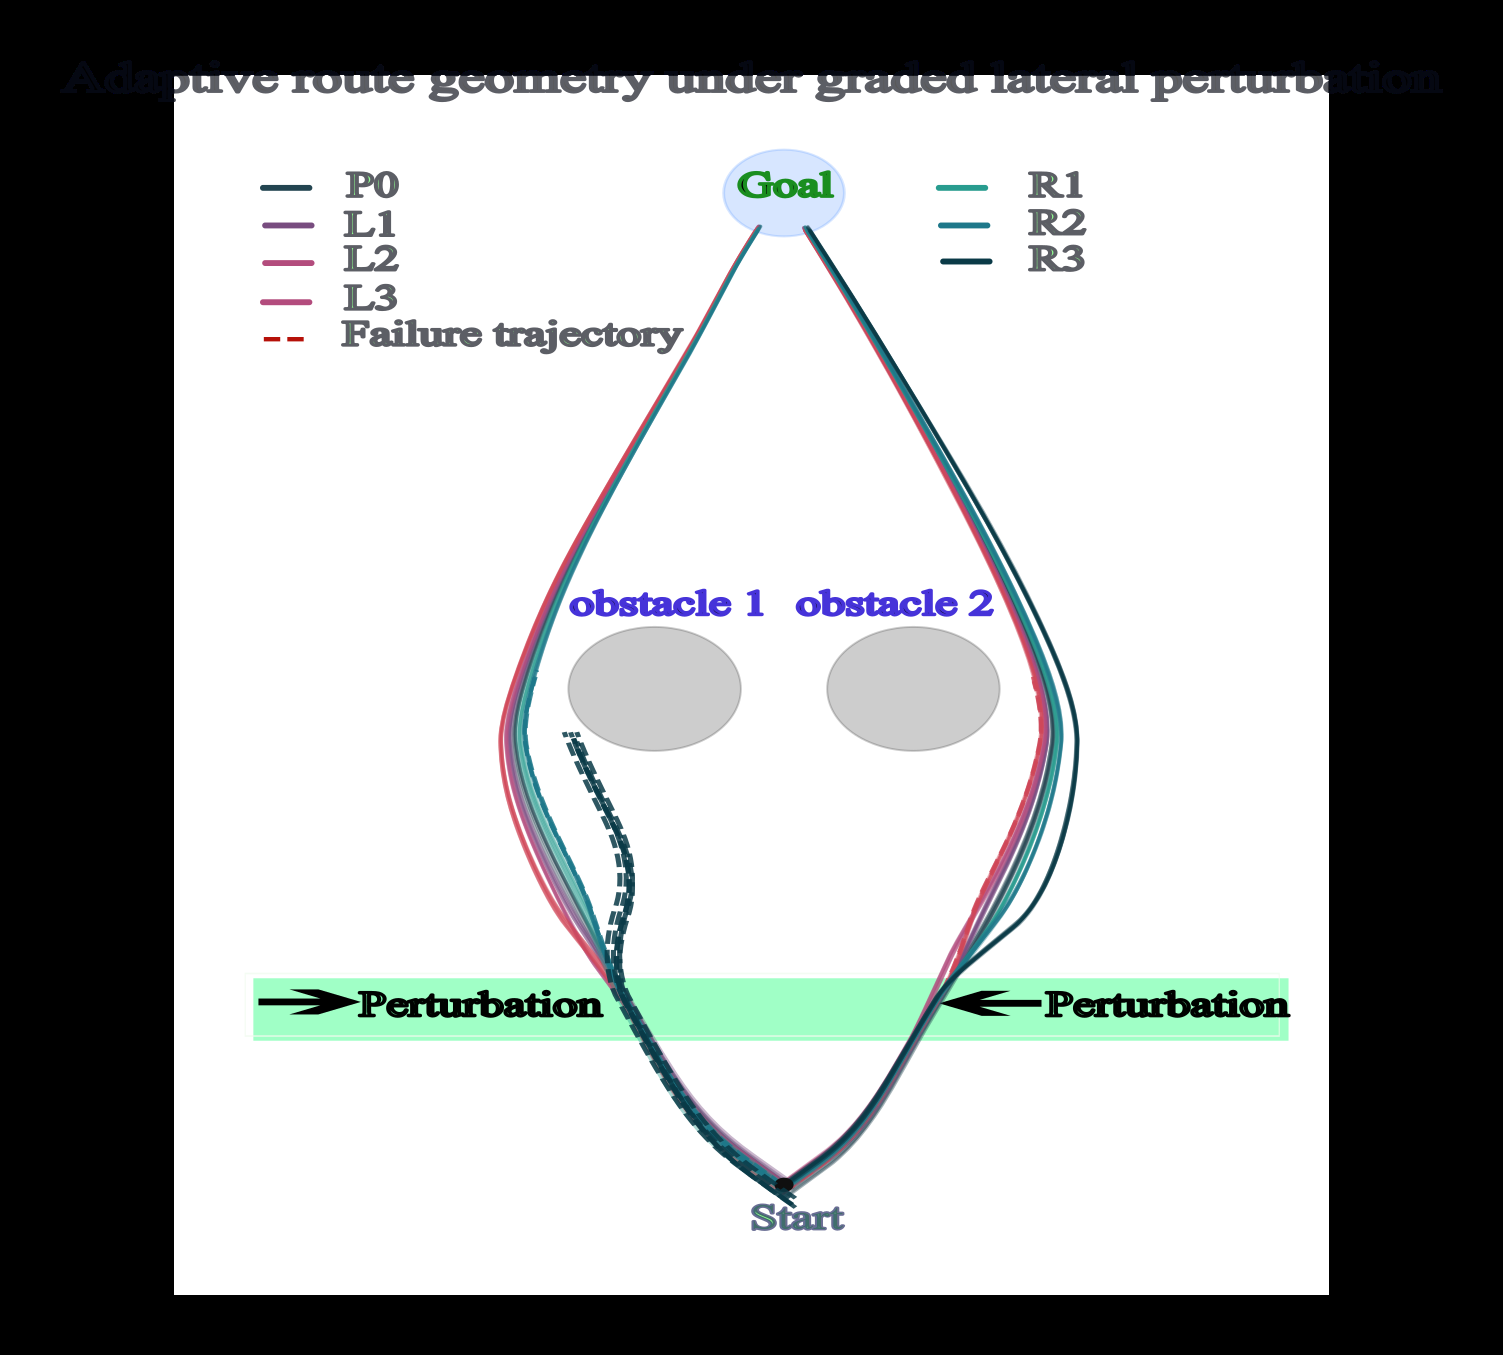
\includegraphics[width=0.60\linewidth]{fig2_trajectories.png}
  \caption{\textbf{Adaptive route geometry under graded lateral
    perturbation.}
    All evaluation episodes are overlaid per condition.
    Solid lines are successful trials; the dashed red line is a failure
    trajectory.
    Leftward conditions (L1--L3, mauve/pink) shift paths left; rightward
    conditions (R1--R3, teal/dark green) shift them right.
    The shaded green band marks the workspace segment where the force
    impulse is applied; grey ellipses are the two static obstacles.
    Goal success was maintained across control and all mild conditions,
    declining only under the two strongest rightward disturbances and the
    strongest leftward impulse, with the rightward direction proving
    disproportionately disruptive.}
  \label{fig:trajectories}
\end{figure}

Failures occurred exclusively under the two strongest rightward conditions
and the largest leftward impulse, with rightward disturbances proving more
disruptive than leftward ones of equal magnitude.
This asymmetry is a geometric consequence of the learned trajectory: it
runs slightly to the left of corridor centre, giving more margin to
absorb leftward pushes before approaching an obstacle boundary.
Across all successful trials, peak speed was effectively invariant across
conditions -- adaptation was achieved through path redirection, not
acceleration.

%--------------------------------------------------------------
\subsection{Kinematic Signatures of Perturbation Direction}
%--------------------------------------------------------------

\begin{figure}[t]
  \centering
  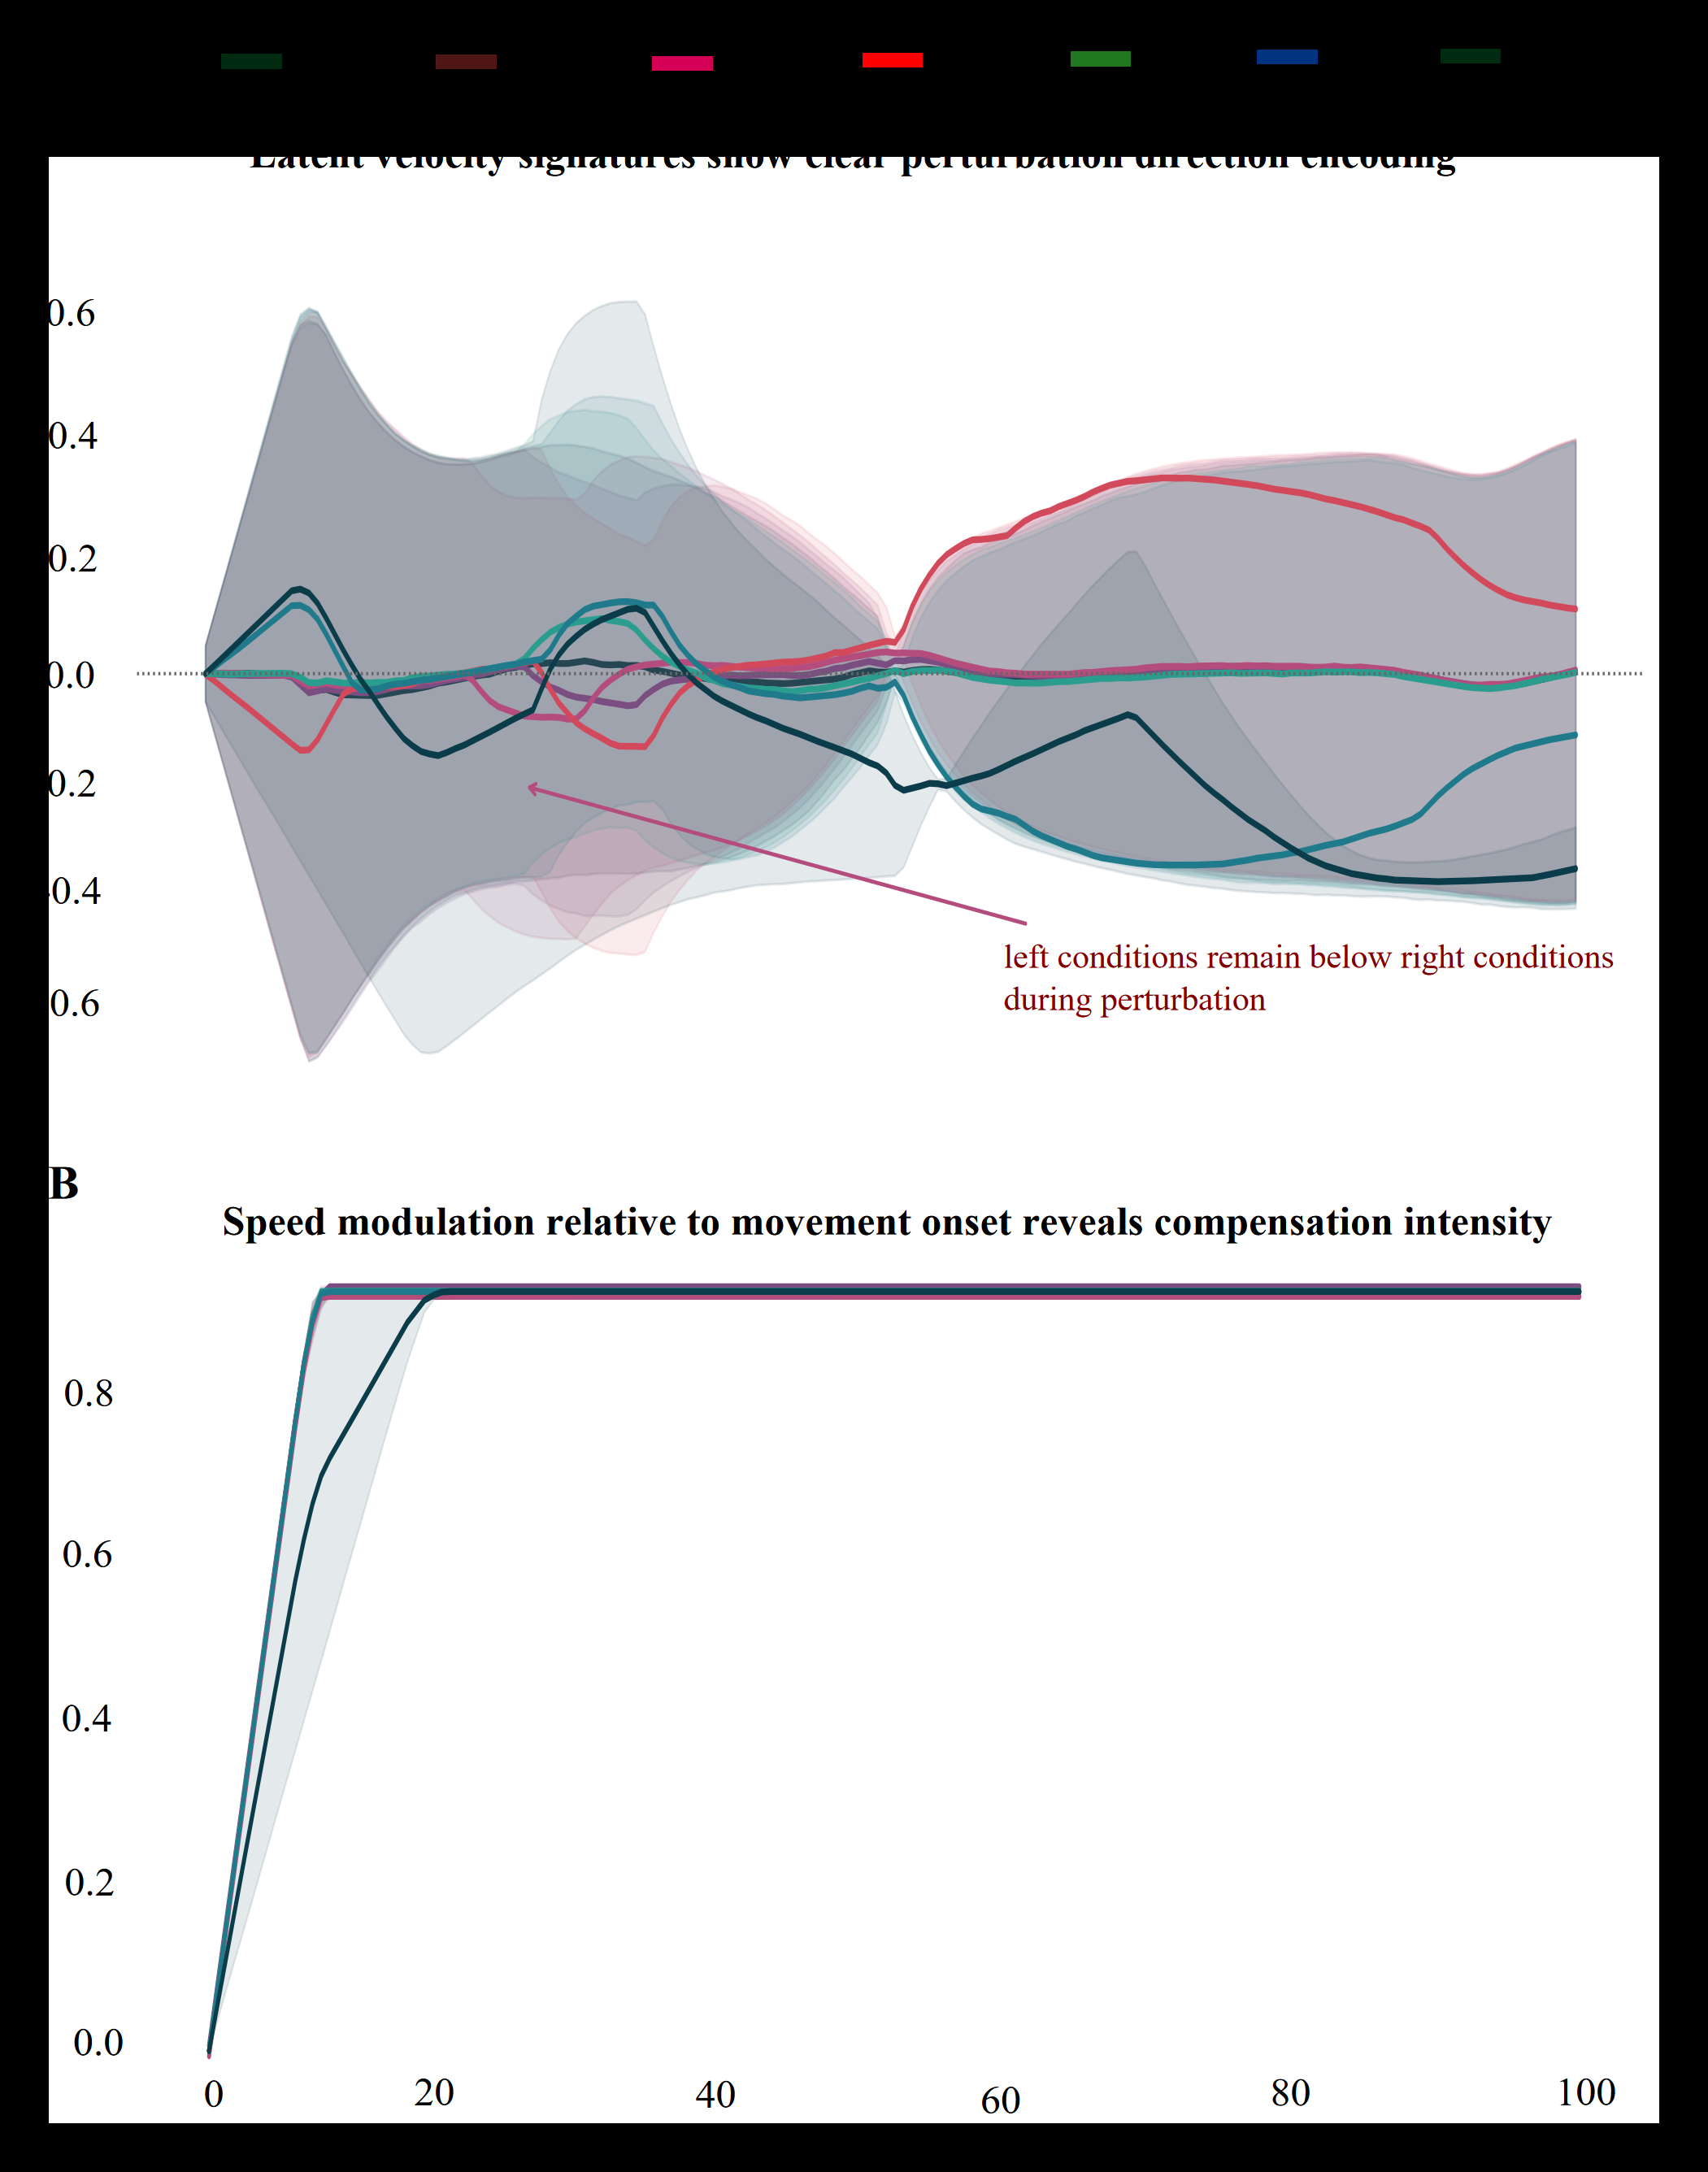
\includegraphics[width=0.80\linewidth]{fig3_velocity.png}
  \caption{\textbf{Velocity profiles across perturbation conditions.}
    \textbf{(A)}~Mean lateral velocity over time (shaded: $\pm$1\,SD).
    Leftward conditions drive negative lateral velocity; rightward drive
    positive. Conditions diverge clearly during the perturbation window
    (timesteps 50--55) and partially reconverge thereafter, consistent
    with a proportional corrective response.
    \textbf{(B)}~Total speed as a function of normalised movement phase.
    Speed rises rapidly at onset and plateaus consistently across all
    seven conditions, confirming that perturbation correction is expressed
    through lateral redirection rather than speed change.}
  \label{fig:velocity}
\end{figure}

Lateral velocity (Figure~\ref{fig:velocity}A) separated cleanly by
direction throughout the perturbation window and scaled with magnitude.
Conditions on the same side of zero partially reconverged afterwards,
indicating a proportional rather than binary corrective response.
Total speed (Figure~\ref{fig:velocity}B) was indistinguishable across
conditions -- the controller preserves movement tempo while redirecting
the path, a kinematic signature consistent with path-correction strategies
in human online reaching
\citep{Pruszynski2012,Nashed2014,FlashHogan1985,Scott2004}.

%--------------------------------------------------------------
\subsection{Low-Dimensional Structure of the Latent State Space}
%--------------------------------------------------------------

\begin{figure}[t]
  \centering
  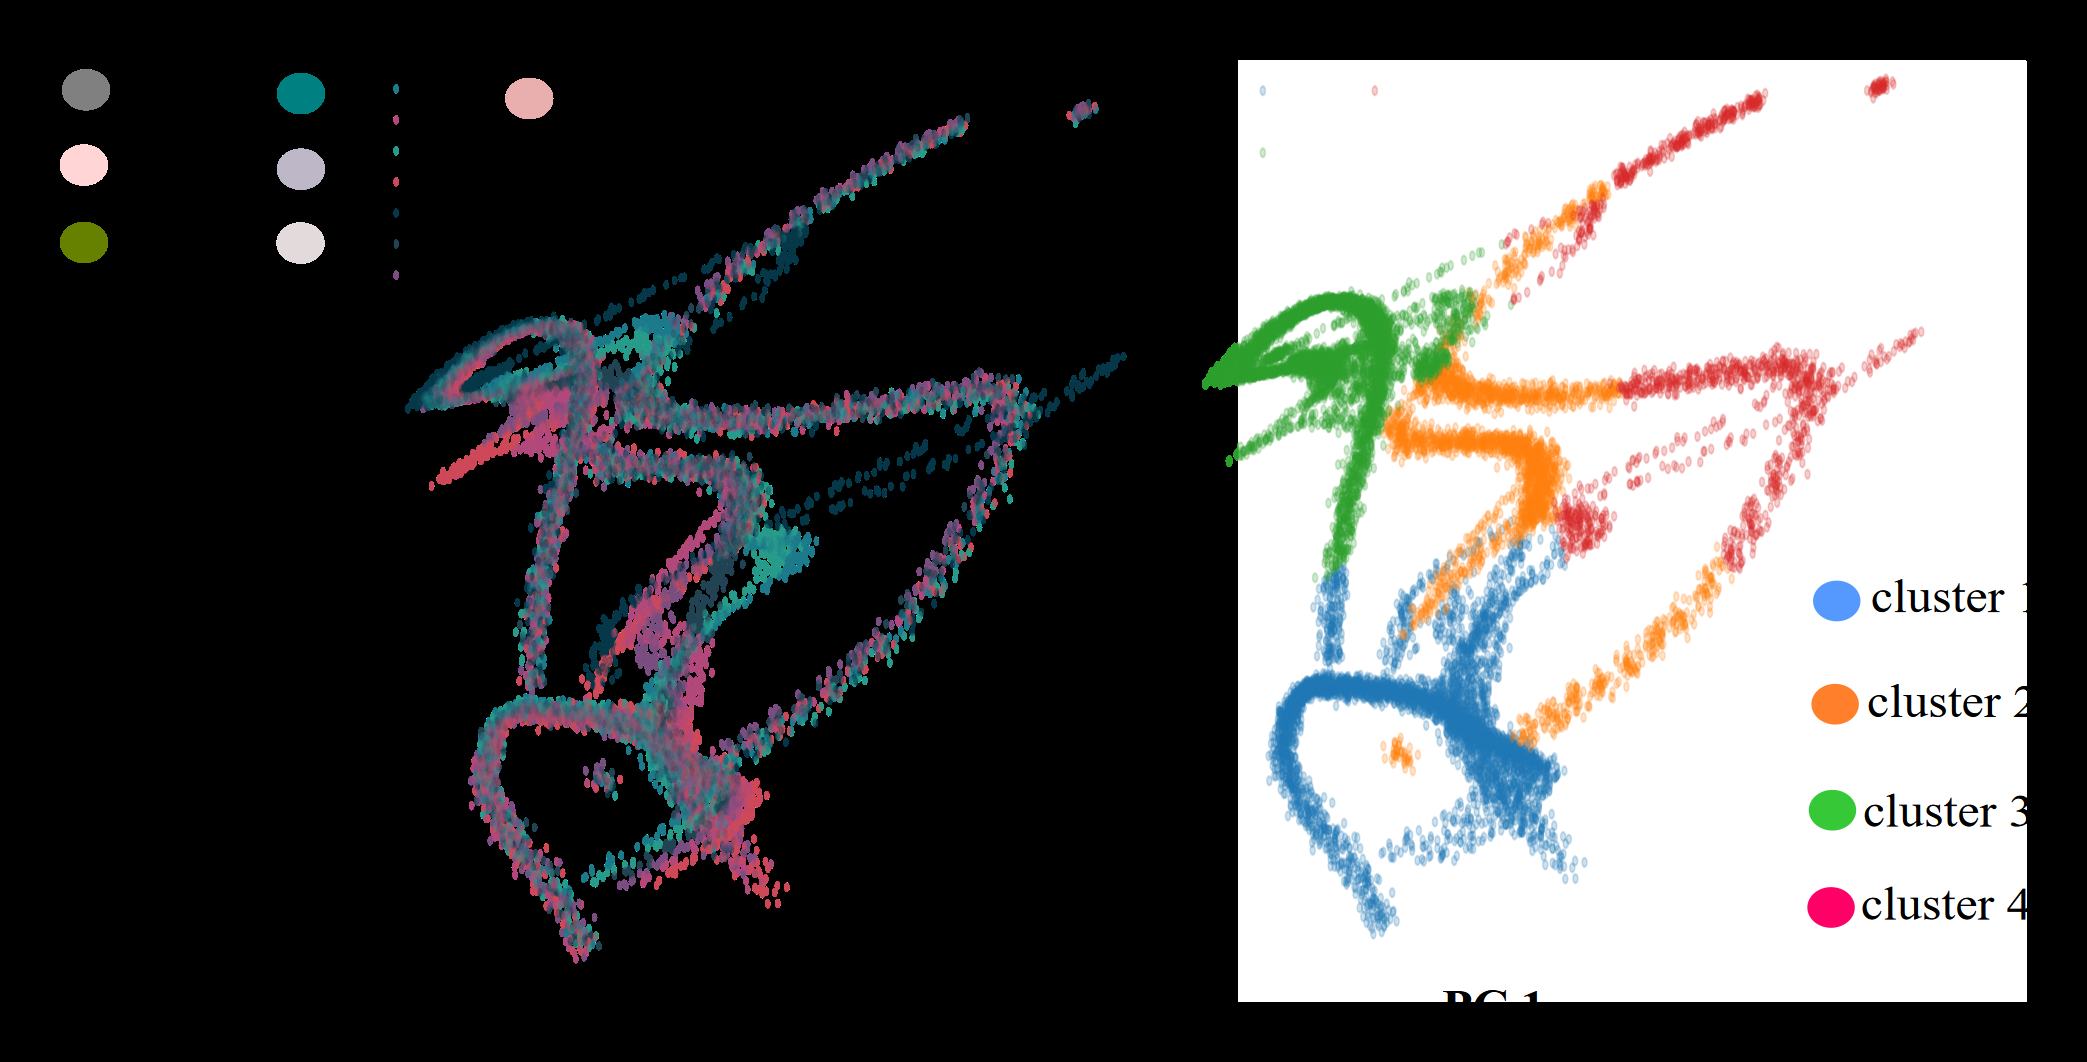
\includegraphics[width=0.90\linewidth]{fig4_pca.png}
  \caption{\textbf{Low-dimensional structure of the policy hidden-layer
    activity.}
    Each point is the 256-dimensional hidden-state at one timestep
    projected onto the first two principal components.
    \textbf{(A)}~Coloured by perturbation condition. The manifold has a
    consistent curved geometry; extreme conditions occupy partially
    separable peripheral regions. PC1 = \PCAVarI{}, PC2 = \PCAVarII{},
    total = \PCAVarTotal{}.
    \textbf{(B)}~Coloured by $K$-means cluster label ($K=4$). The
    manifold divides into four spatially coherent regions likely
    corresponding to movement phases -- approach, perturbation,
    correction, arrival -- shared across all conditions.}
  \label{fig:pca}
\end{figure}

Two findings stand out from the PCA
(Figure~\ref{fig:pca}).
First, \PCAVarTotal{} of the variance in a 256-unit network is captured
by two dimensions alone, indicating a compact low-dimensional
representation consistent with neural manifold structure in motor cortex
\citep{Churchland2012,Shenoy2013,Cunningham2014,Gallego2017}.
Second, the manifold subdivides into four spatially coherent clusters
that do not align with individual perturbation conditions; they likely
reflect discrete movement phases shared across all trials.
Perturbation-specific differences appear as density shifts within this
shared geometry rather than as separate manifolds, suggesting a common
computational substrate for obstacle avoidance that is modulated by
perturbation context.

%--------------------------------------------------------------
\subsection{Linear Decoding of Perturbation Context}
%--------------------------------------------------------------

\begin{figure}[t]
  \centering
  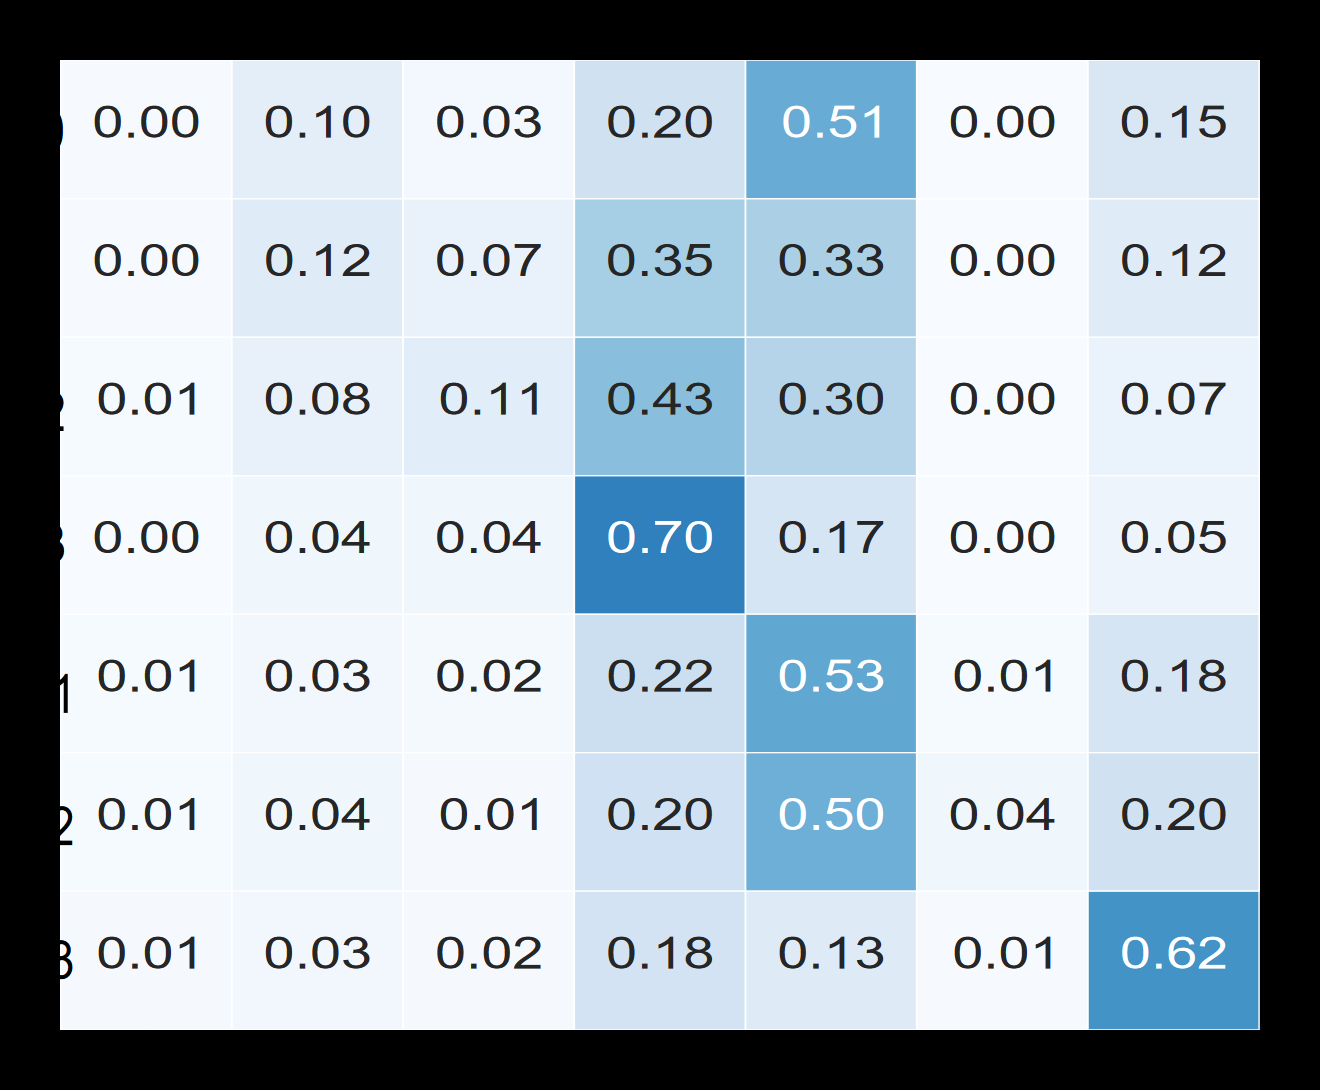
\includegraphics[width=0.55\linewidth]{fig5_decoding.png}
  \caption{\textbf{Linear decoding of perturbation condition from
    hidden-layer activity.}
    Rows are the true condition; columns are the classifier's prediction.
    Diagonal entries (darker blue) are correct classifications.
    The largest leftward (L3) and rightward (R3) conditions are decoded
    most reliably. The unperturbed control and mild leftward conditions
    are frequently predicted as L3, reflecting their geometric proximity
    to the L3 cluster in the latent manifold rather than a simple decoding
    failure.}
  \label{fig:decoding}
\end{figure}

A linear classifier trained on single-timestep hidden activity
(Figure~\ref{fig:decoding}) decoded the most extreme perturbation
conditions most accurately: the largest leftward impulse was correctly
identified in roughly seven out of ten timesteps, and the largest
rightward impulse in roughly six out of ten.
Moderate rightward conditions were also decoded above chance.
The unperturbed control and mild leftward conditions were most often
misclassified as the largest leftward condition, reflecting their
geometric proximity in the manifold.
The success of linear decoding at all indicates that perturbation context
is encoded in a geometrically structured, directly accessible form --
not buried in nonlinear interactions among units -- mirroring the linear
decodability of task context from motor cortex population activity during
biological reaching \citep{Churchland2012,Nashed2014,Oby2019}.

%--------------------------------------------------------------
\subsection{Learning Trajectory and Stability}
%--------------------------------------------------------------

\begin{figure}[t]
  \centering
  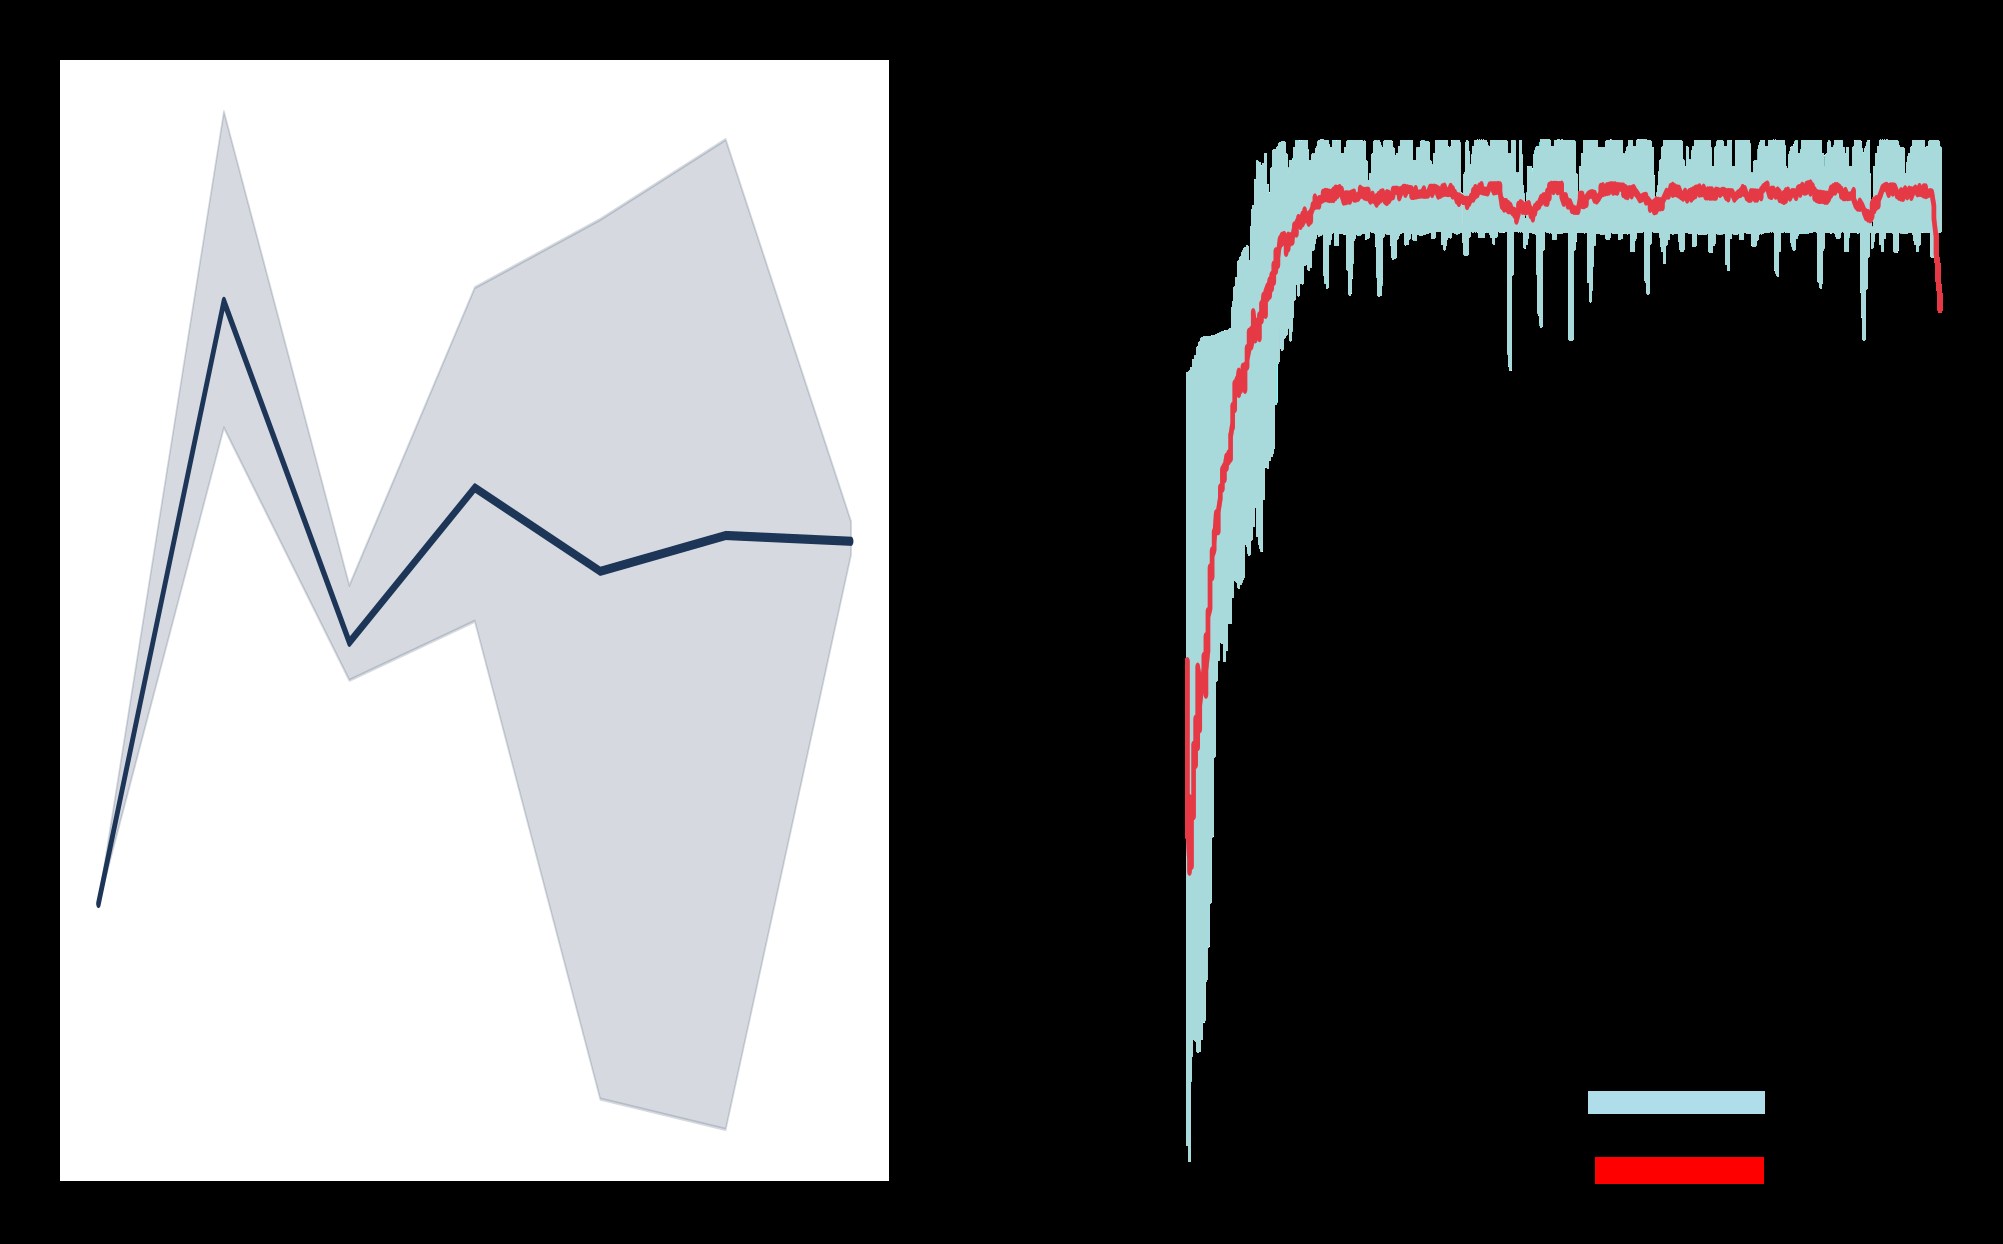
\includegraphics[width=0.82\linewidth]{fig6_learning.png}
  \caption{\textbf{Learning stability and policy improvement.}
    \textbf{(Left)}~Evaluation reward across training checkpoints
    (mean $\pm$\,SD) showing stable performance after convergence.
    \textbf{(Right)}~Episode reward over the full training run: raw
    per-episode values (light blue) and a smoothed trace (red) confirm
    rapid improvement in the first third of training and a stable plateau
    thereafter. The representations analysed in
    Figures~\ref{fig:pca}--\ref{fig:decoding} were extracted from this
    converged policy.}
  \label{fig:learning}
\end{figure}

Reward rose rapidly within the first third of the training budget and
then plateaued stably (Figure~\ref{fig:learning}).
Evaluation reward across independently sampled checkpoints was tightly
distributed around the plateau value, confirming that the representational
analyses in Sections~3.3 and~3.4 reflect a well-converged rather than
partially-trained controller.

%==============================================================
\section{Discussion}
%==============================================================

This study asked whether a PPO controller trained for adaptive obstacle
avoidance develops internal representations that are interpretable in
the same terms used to study biological motor populations.
Across behaviour, kinematics, latent geometry, and linear decodability,
the findings are consistently affirmative -- with qualifications that
deserve careful statement.

\paragraph{Behavioural adaptation mirrors biological feedback correction.}
The controller maintained robust performance under mild perturbations and
degraded progressively under stronger ones, with a direction-dependent
asymmetry attributable to the geometry of the learned corridor trajectory.
Critically, the movement tempo -- measured by total speed -- was preserved
across all conditions; adaptation appeared entirely in path geometry.
This separation between corrective redirection and preserved speed is the
same kinematic signature documented for online feedback corrections in
human reaching, where motor cortex updates movement direction without
imposing systematic speed changes
\citep{Pruszynski2012,Nashed2014,FlashHogan1985,Scott2004,Dimitriou2013}.
We do not claim that the controller mimics a biological motor system; its
dynamics are far simpler than those of a real limb, and it was optimised
for reward rather than biological fidelity.
Nevertheless, the convergence of the kinematic signature is consistent
with optimal feedback control principles
\citep{Todorov2002,Todorov2009} and suggests that this particular
strategy may be a computationally preferred solution whenever a system
must redirect a moving body under time pressure.

\paragraph{Low-dimensional latent structure and its biological parallel.}
The finding that the majority of variance in a 256-unit network collapses
onto two dimensions is notable because the network was never constrained
to be low-dimensional.
In biological motor cortex, the dominant computational subspace during
reaching spans far fewer dimensions than the number of recorded neurons,
a property attributed to the structured, repetitive nature of movement
\citep{Churchland2012,Shenoy2013,Cunningham2014,Gallego2017,Blohm2009,Blohm2012}.
Our results suggest that a similar pressure operates in reward-driven
learning: because successful reaches share a common temporal structure,
the network represents the essential state of the movement compactly,
with perturbation context appearing as a modulation of shared geometry.
The four-cluster decomposition reinforces this: the clusters align with
movement phases rather than conditions, consistent with phase-structured
dynamics in motor cortex \citep{Churchland2012,Shenoy2013}.
We note that the $K=4$ solution was identified post hoc; replication
across multiple training seeds and held-out data would be needed to
confirm whether this is a stable feature of the learned representation.

\paragraph{Decoding and what it implies about internal organisation.}
The pattern of decoder performance -- reliable for extreme conditions,
near-chance for mild ones -- is not a simple decoding failure.
It is a property of the manifold geometry: mild perturbations generate
hidden states that are geometrically indistinguishable from larger
perturbations that were also well corrected, because the controller
handled them with similar small adjustments.
This has a direct parallel in biological motor cortex, where the
decodability of perturbation magnitude improves when classifiers are given
a temporal window of population activity rather than a single snapshot
\citep{Nashed2014,Churchland2012}.
The practical implication for both artificial and biological systems is
that a single snapshot of population activity is not always sufficient to
identify the perturbation magnitude; understanding the source of
failure requires following the representational trajectory over time.

\paragraph{Limitations.}
Results are from a single training seed; variability across runs is
unknown.
The environment is simplified: two-dimensional, static obstacles, a fixed
perturbation window, and point-mass dynamics far simpler than a real limb.
The feedforward MLP has no recurrence, limiting its ability to maintain
a running internal estimate of perturbation history.
PCA and decoding are descriptive; they confirm that structure exists but
do not establish causal links between specific units and behaviour.
Large language models were used to support editing, proofreading, and
\LaTeX\ formatting; they were not used to generate data, run analyses,
or draw scientific conclusions.

\paragraph{Implications for biological and artificial systems.}
Our results contribute to growing evidence that the organisational
principles of biological motor populations -- compact manifold geometry,
phase-structured latent dynamics, and linear decodability of task context
-- are not unique to neural circuits shaped by evolution and development.
They can emerge spontaneously from reward-driven optimisation in
artificial networks
\citep{Churchland2012,Gallego2017,Oby2019,Crevecoeur2019,Blohm2009}.
This convergence is meaningful in two directions.
For neuroscientists, it validates using neuroscience-inspired analytical
tools on artificial controllers, enabling the same interpretive language
applied to motor cortex to be used for autonomous systems.
For engineers and clinicians working on assistive or rehabilitation
technologies -- where understanding the relationship between internal
representations, behavioural adaptation, and movement recovery is
practically important -- it suggests that these analytical tools may
provide actionable diagnostic information beyond simple task-success
metrics.
Understanding where and how representational structure breaks down under
strong perturbations could inform both our understanding of motor cortex
failure modes and the design of more robust, interpretable controllers.

%==============================================================
\section{Conclusion}
%==============================================================

We trained a PPO controller on an obstacle-avoidance reaching task and
analysed its internal representations using the population-level toolkit
of motor neuroscience.
The controller adapted to moderate perturbations through path-level
corrections that preserved movement speed, with robustness declining
asymmetrically under strong rightward disturbances.
The hidden-layer activity organised into a compact low-dimensional
manifold -- capturing the large majority of population variance in two
dimensions -- with four phase-aligned clusters shared across conditions.
Extreme perturbation conditions produced latent states separable by a
linear classifier; mild conditions did not, a pattern mirroring
difficulty-dependent decodability in biological motor cortex.

These findings demonstrate that reward-driven learning generates
structured internal representations with organisational properties
consistent with biological motor populations.
Treating policy hidden activity as a population signal extends behavioural
evaluation and may help explain why adaptive controllers succeed or fail
under conditions they were not explicitly trained on.
Future work will extend this framework to recurrent architectures, richer
environments, and multiple training seeds, and will test whether the
representational structure identified here predicts behavioural failure
across task variants.

%==============================================================
\section*{Acknowledgments}
%==============================================================

This work was supported in part by the Connected Minds Program,
Canada First Research Excellence Fund,
Grant No.~CFREF-2022-00010.

\bibliographystyle{unsrtnat}
\bibliography{references}

\end{document}
